\documentclass[tikz,border=1pt]{standalone}
\usepackage{amsmath,amssymb,bm}
\usepackage{tikz}
\usetikzlibrary{decorations.pathmorphing,patterns}


\usepackage{tikz}
\usepackage{tikz}
\usepackage{pgfplots}
\usetikzlibrary{decorations.pathmorphing,patterns}

\usetikzlibrary{
    spath3,
    intersections,
    arrows,
    knots,
    calc,
    hobby,
    decorations.pathreplacing,
    shapes.geometric,
}

% ---------------- Global styles (safe for 'knots') ----------------
\tikzset{
    knot diagram/every strand/.append style={
        line cap=round,
        line join=round,
        ultra thick,
        black
    },
    every knot/.style={line cap=round,line join=round,very thick},
    strand/.style={line cap=round,line join=round,line width=3pt,draw=black},
    over/.style={preaction={draw=white,line width=6.5pt}},
% DO NOT set a global "every path" here; it breaks internal clip paths.
}
% ------- TikZ Guide Lines -------
\newcommand{\SSTGuidesPoints}[2]{% #1=basename (e.g. P), #2=last index
    \foreach \i in {1,...,#2}{
      \fill[blue] (#1\i) circle (1.2pt);
      \node[blue,font=\scriptsize,above] at (#1\i) {\i};
    }
    \draw[gray!40, dashed]
    \foreach \i [remember=\i as \lasti (initially 1)] in {2,...,#2,1} { (#1\lasti)--(#1\i) };
}
\providecommand{\swirlarrow}{\rightsquigarrow}
\begin{document}
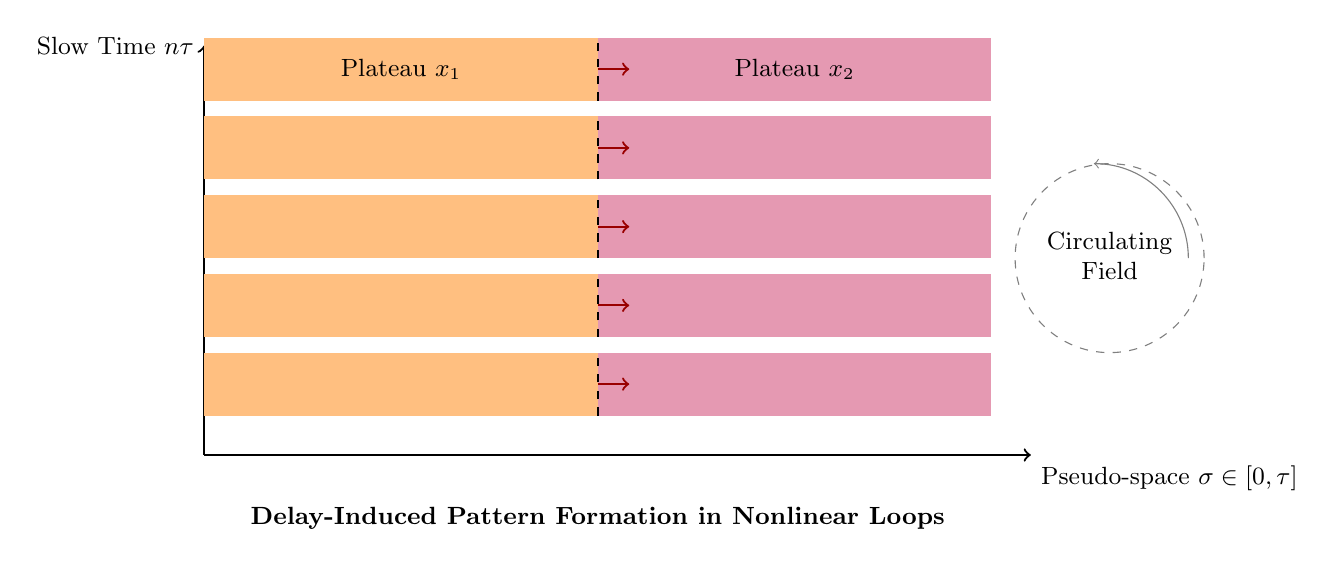
\begin{tikzpicture}
\draw[->, thick] (0,0) -- (0,5.2) node[left] {\small Slow Time $n\tau$};
        \draw[->, thick] (0,0) -- (10.5,0) node[below right] {\small Pseudo-space $\sigma \in [0,\tau]$};


        \foreach \y in {0.5,1.5,...,4.5} {
            \fill[orange!50] (0,\y) rectangle (5,\y+0.8);
            \fill[purple!40] (5,\y) rectangle (10,\y+0.8);
            \draw[dashed, thick] (5,\y) -- (5,\y+0.8); 
        }


        \node at (2.5,4.9) {\small Plateau $x_1$};
        \node at (7.5,4.9) {\small Plateau $x_2$};


        \foreach \y in {0.5,1.5,...,4.5} {
            \draw[->, thick, red!60!black] (5,\y+0.4) -- (5.4,\y+0.4);
        }


        \draw[dashed, gray] (11.5,2.5) circle(1.2);
        \node at (11.5,2.5) {\small \begin{tabular}{c}Circulating\\Field\end{tabular}};
        \draw[->, gray] (12.5,2.5) arc[start angle=0,end angle=90,radius=1.2];


        \node[align=center] at (5,-0.8) {\small \textbf{Delay-Induced Pattern Formation in Nonlinear Loops}};
\end{tikzpicture}
\end{document}